
\documentclass{article}
\usepackage{amsmath}
\usepackage[margin=1in]{geometry}
\usepackage{amsfonts}
\usepackage{hyperref}
\usepackage{graphicx}
\usepackage{siunitx}
\usepackage{cancel}


\begin{document}

\title{Essence of Single Variable Calculus}
\author{Andy Chong Sam}
\date{}
\maketitle

\section{Derivatives}

\par \noindent We will first summarize derivatives. Given a function \( f(x)\), its derivative \(f'(x)\), describes the instantaneous rate of change at \(x\).
The formal definition of the derivative is as follows:

\begin{flalign*}
	f'(x) = \lim_{\Delta x \to  0 } \frac{f(x+ \Delta x) - f(x)}{\Delta x}
\end{flalign*}

\par\noindent From the expression above we can derive all the derivatives found on a textbook table.

\section{Integrals}


\begin{minipage}{.6\linewidth}		
	
	\par \noindent A definite integral across a continuous interval \([a,b]\) is defined as:
	
\begin{flalign*}
	\int_{a}^{b} f(x) dx = \lim_{n \to  \infty } \sum_{i=1}^{n} f(t) \Delta x
\end{flalign*}
	
	\begin{center}
		t is a point within an interval of width \(\Delta x\)
	\end{center}

	\par \noindent From a practical standpoint, the definite integral tells us the area under the curve from point \(a\) to \(b\). 
	\newline
	\par\noindent In Figure 1, we try and approximate the area under \(x^2\) for the interval \([0,1]\) by creating rectangles with heights of \(f(t)\) and width of \( \Delta x\). Using more rectangles, with smaller values of \( \Delta x\) gets us an increasingly accurate measure of the area.

\end{minipage}
\begin{minipage}[c]{.4\linewidth}
	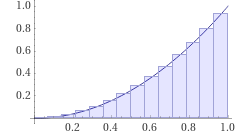
\includegraphics[width=7cm]{rsum.png}
	
	\begin{center}
		Figure 1
	\end{center}
	
\end{minipage}
\newline
\newline
\par \noindent Given a function \(f(x)\) and \(F(x)\), if \(F'(x) = f(x)\) then we say that \(F(x)\) is the anti-derivative of \(f(x)\). This is one key connection between derivatives and integrals. Now we can define an \textbf{indefinite integral} as:

\begin{flalign*}
	\int f(x) dx = F(x) + C
\end{flalign*}

\par \noindent In this expression \(C\) is an arbitrary constant. This is needed for the following situation: Suppose we have \(x^2 + 3\) or \(x^2 + 5\), taking the derivative of either expression will result in \(2x\).
\newline
\par \noindent Using the Second Fundamental Theorem of Calculus, which we will discuss later, the \textbf{definite integral} can be defined as:

\begin{flalign*}
	\int_{a}^{b} f(x) dx = F(b) - F(a) 
\end{flalign*}


\section{Mean Value Theorem}
\begin{minipage}{.6\linewidth}		

\par \noindent Given a continuous function \(f\) on a closed interval \([a,b]\), then there is a point \(c\), such that \(f'(c)\) is equivalent to the slope of the secant line that runs from points \(a\) and \(b\). 

\begin{flalign*}
	\frac{f(b)-f(a)}{b-a} = f'(c)
\end{flalign*}

	\par\noindent In Figure 2 the line that runs through points \(a\) and \(b\) has the same slope as the tangent line that runs through point \(c\)



	
\end{minipage}
\begin{minipage}[c]{.4\linewidth}
	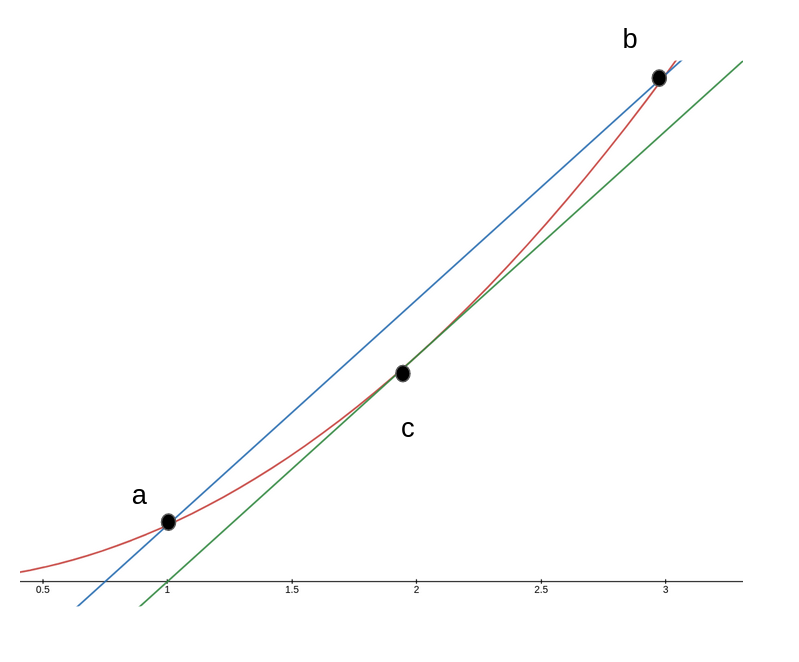
\includegraphics[width=7cm]{sec.png}
	
	\begin{center}
		Figure 2
	\end{center}
	

\end{minipage}

\section {Mean Value Theorem of Integrals}

\begin{minipage}{.6\linewidth}		

\par \noindent Given a continuous function \(f\) there exists a value \(c\) such that

\begin{flalign*}
	\int_{a}^{b} f(x) dx = f(c)(b-a)
\end{flalign*}

	\par\noindent In Figure 3 the mean value theorem of integrals predicts that the area under the curve from points a to b is equivalent to the purple edged rectangle with a height of \(f(c)\) and length \(b-a\).
 	
	
\end{minipage}
\begin{minipage}[c]{.4\linewidth}
		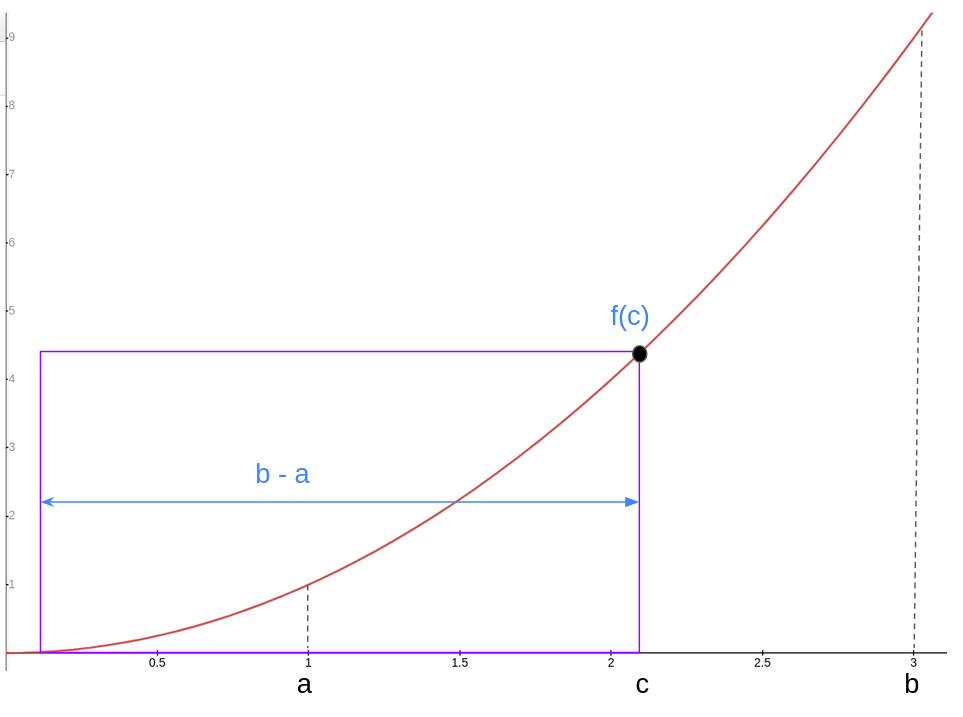
\includegraphics[width=7cm]{mvt-int.png}
	
	\begin{center}
		Figure 3
	\end{center}
	

	
\end{minipage}


\section{First Fundamental Theorem of Calculus}

\par \noindent \textbf{If \(f(x)\) is continuous over \([a,b]\), and \(F(x) = \int_{a}^{x} f(t) dt \), then \(F'(x)=f(x)\) over \([a,b]\).} We say that \(F\) is an antiderivative of \(f\).
\newline
\par\noindent\textbf{Derivation:}
\newline
\begin{flalign*}
	F'(x) = \lim_{\Delta x \to  0 } \frac{F(x+ \Delta x) - F(x)}{\Delta x} \\ \\
	F'(x) = \lim_{\Delta x \to  0 } \frac{\int_{a}^{x + \Delta x}f(t)dt - \int_{a}^{x}f(t)dt}{\Delta x} \\ \\
	F'(x) = \lim_{\Delta x \to  0 } \frac{\int_{x}^{x + \Delta x}f(t)dt}{\Delta x}
\end{flalign*}
\par\noindent By the \textbf{Mean Value Theorem of Integrals} we know that there is a value \(c\) such that:

\begin{flalign*}
f(c) \Delta x = \int_{x}^{x + \Delta x}f(t)dt
\end{flalign*}

\par \noindent We are left with evaluating:

\begin{flalign*}
F'(x)= \lim_{\Delta x \to  0 } f(c) \Delta x
\end{flalign*}

\par \noindent By the \textbf{Squeeze Theorem} we know that as \(\Delta x\) approaches zero, \(c\) approaches \(x\), so we are left with:

\begin{flalign*}
	F'(x) = \lim_{\Delta x \to  0 } f(c) \Delta x = f(x)
\end{flalign*}

\newpage

\section {Second Fundamental Theorem of Calculus}

\par\noindent \textbf{If \(f(x)\) is continuous over \([a,b]\), then \(\int_{a}^{b} f(x) dx = F(b) - F(a)\)}.
\newline
\par\noindent \textbf{Derivation:}
\newline
\par\noindent There are infinite real numbers between \(a\) and \(b\), so we can say that:

\begin{flalign*}
	a = x_0 < x_1 < x_2 < ... < x_{n-1} < x_n = b
\end{flalign*}

\par\noindent We can replace \(a\) and \(b\) with \(x_0\) and \(x_n\) respectively:

\begin{flalign*}
	F(b) - F(a) = F(x_n) - F(x_0)
\end{flalign*}

\par\noindent Next, we insert a series of self-cancelling expressions:

\begin{flalign*}
	F(b) - F(a) = F(x_n) + (-F(x_{n-1}) + F(x_{n-1})) +  (-F(x_{n-2}) + F(x_{n-2})) + ... + (-F(x_1) + F(x_1)) - F(x_0) \\
	=(F(x_n) - F(x_{n-1})) +  (F(x_{n-1}) - F(x_{n-2})) + ... + (F(x_2) - F(x_1)) + (F(x_1) - F(x_0))
\end{flalign*}

\par \noindent This result can be summarized with the summation:

\begin{flalign*}
		F(b) - F(a) = \sum_{i=1}^{n} (\;\;F(x_i) - F(x_{i-1})\;\;)
\end{flalign*}

\par\noindent By the Mean Value Theorem of Integrals we know that there is a value \(c\) such that \\ \(F(x_i) - F(x_{i-1}) = F'(c)(x_i - x_{i-1})\). We can now rewrite \(F(b) - F(a)\) as:

\begin{flalign*}
F(b) - F(a) = \sum_{i=1}^{n} (\;\;F'(c)(x_i - x_{i-1})\;\;)
\end{flalign*} 

\par\noindent By the First Fundamental Theorem of Calculus we know that \(F'(c) = f(c)\) so we now have:

\begin{flalign*}
F(b) - F(a) = \sum_{i=1}^{n} (\;\;f(c)(x_i - x_{i-1})\;\;)
\end{flalign*}

\par\noindent If we take the limit for both sides we will be left with definition of the definite integral on the right hand side. This is the same definition we saw in section 2:

\begin{flalign*}
	\lim_{n \to  \infty } (\;\;F(b) - F(a)\;\;) = \lim_{n \to  \infty } \sum_{i=1}^{n} (\;\;f(c)(x_i - x_{i-1})\;\;) \\
	F(b) - F(a) = \lim_{n \to  \infty } \sum_{i=1}^{n} (\;\;f(c)(x_i - x_{i-1})\;\;)
\end{flalign*}

\par\noindent We are left with:

\begin{flalign*}
	\int_{a}^{b} f(x) dx = F(b) - F(a) 
\end{flalign*}

\newpage
\section{Product Rule}

\par\noindent Given \(h(x) = f(x)g(x)\), \(h'(x) = f'(x)g(x) + f(x)g'(x)\)

\begin{flalign*}
	h'(x) = \lim_{h \to  0 }\frac{f(x+h)g(x+h) - f(x)g(x)}{h}
\end{flalign*}

\par\noindent We'll add the following two terms which cancel each other out, \(-f(x+h)g(x) + f(x+h)g(x)\):

\begin{flalign*}
		h'(x) = \lim_{h \to  0 }\frac{f(x+h)g(x+h) -f(x+h)g(x) + f(x+h)g(x) - f(x)g(x)}{h} \\
		= \lim_{h \to  0 }\frac{f(x+h)(g(x+h) - g(x)) + g(x)(f(x+h)-f(x))}{h} \\
		= \lim_{h \to  0 }\frac{f(x+h)(g(x+h) - g(x))}{h} + \lim_{h \to  0 }\frac{g(x)(f(x+h))-f(x)}{h} \\
\end{flalign*}

\par\noindent The limit \(\lim_{h \to  0 } f(x+h)\) is just \(f(x)\). We can also see that \(\lim_{h \to  0 } \frac{g(x+h)-g(x)}{h}\) is \(g'(x)\).
\newline
\par\noindent We also observe that \(\lim_{h \to  0 }g(x) = g(x)\) and \(\lim_{h \to  0 }\frac{f(x+h) - f(x)}{h}\) is the definition of \(f'(x)\).

\section{Quotient Rule}

\par\noindent If \(h(x) = \frac{f(x)}{g(x)}\) then \(h'(x) = \frac{f'(x)g(x) - f(x)g'(x)}{g(x)^2}\)
\newline

\par\noindent We will apply the cross multiplication property. Given \(\frac{a}{b} - \frac{c}{d} = \frac{ad-bc}{bd}\):

\begin{flalign*}
	h'(x) = \lim_{h \to  0 } \frac{\frac{f(x+h)}{g(x+h)} - \frac{f(x)}{g(x)}}{h} \\
	=\lim_{h \to  0 } \frac{f(x+h)g(x) - f(x)g(x+h)}{g(x+h)g(x)}\;\frac{1}{h}
\end{flalign*}

\par\noindent We'll add to the numerator two terms that cancel each other out \(-f(x)g(x) + f(x)g(x)\):

\begin{flalign*}
	h'(x)=\lim_{h \to  0 } \frac{f(x+h)g(x) -f(x)g(x) + f(x)g(x) - f(x)g(x+h)}{g(x+h)g(x)}\;\frac{1}{h} \\
	= \lim_{h \to  0 } \frac{1}{g(x+h)g(x)}\frac{f(x+h)g(x) -f(x)g(x) + f(x)g(x) - f(x)g(x+h)}{h} \\
	= \lim_{h \to  0 } \frac{1}{g(x+h)g(x)} ( \frac{f(x+h)g(x) - f(x)g(x)}{h} + \frac{f(x)g(x) - f(x)g(x+h)}{h}) \\
	= \lim_{h \to  0 } \frac{1}{g(x+h)g(x)} ( g(x)\frac{f(x+h) - f(x)}{h} + f(x)\frac{g(x) - g(x+h)}{h})
\end{flalign*}

\par \noindent From these results we can see that: 
\newline
\par\noindent \(\lim_{h \to  0 } \frac{1}{g(x+h)g(x)}\) is \( \frac{1}{g(x)^2}\)
\newline
\par \noindent \( \lim_{h \to  0 }g(x)\frac{f(x+h) - f(x)}{h}\) is \(g(x)f'(x)\).
\newline
\par \noindent \( \lim_{h \to  0 }f(x)\frac{g(x+h) - g(x)}{h}\) is \(f(x)g'(x)\).
\newpage

\section {Chain Rule}

\par \noindent Given a composition relationship \(h(x) = f(g(x))\) then \(h'(x) = f'(g(x))g'(x)\). 
\newline
\par \noindent Let's suppose that we're interested in the derivative at a specific point \(a\), so we can say:

\begin{flalign*}
	\lim_{x \to  a } \frac{f(g(x)) - f(g(a))}{x-a}
\end{flalign*}

\par \noindent If we multiply the entire expression by \(\frac{g(x)-g(a)}{g(x)-g(a)}\):

\begin{flalign*}
	\lim_{x \to  a } \frac{f(g(x)) - f(g(a))}{x-a}\;\; \frac{g(x)-g(a)}{g(x)-g(a)} \\
	= \lim_{x \to  a } \frac{f(g(x)) - f(g(a))}{g(x)-g(a)} \;\; \frac{g(x)-g(a)}{x-a}
\end{flalign*}

\par\noindent The left fraction corresponds to the rate of change \(f'(g(a))\), while the right fraction corresponds to the rate of change \(g'(a)\)


\section {Power Rule}

\par\noindent Given \(f(x) = x^n\), its derivative is \(f'(x) = nx^{n-1}\)
\newline
\par\noindent \textbf{Derivation:}
\begin{flalign*}
	f'(x) = \lim_{h \to  0 } \frac{(x+h)^n - x^n}{h}
\end{flalign*}
\par\noindent By the Binomial Theorem, we know that:
\begin{flalign*}
	(a+b)^n = \sum_{k=0}^{n} \frac{n!}{k!(n-k)!} a^{n-k}b^k
\end{flalign*}
\par\noindent Expanding the numerator we have:
\begin{flalign*}
	f'(x)= \lim_{h \to  0 } \frac{(x^n + nx^{n-1}h + \frac{n(n-1)}{2!}x^{n-2}h^2 + ... + nxh^{n-1} + h^n) - x^n}{h} \\
	= \lim_{h \to  0 } (nx^{n-1} + \frac{(n)(n-1)}{2!}x^{n-2}h + ... + nxh^{n-2} + h^{n-1})
\end{flalign*}
\par\noindent With the exception of \(n(x)^{n-1}\), the limit as \(h\) approaches zero of all other components is zero, for instance:


\begin{flalign*}
	\lim_{h \to  0 } (\frac{(n)(n-1)}{2!}x^{n-2}h) = 0 \;\;\;\;\;
	\lim_{h \to  0 } (nxh^{n-2}h) = 0 \;\;\;\;\;
	\lim_{h \to  0 } (h^{n-1}) = 0 \\
\end{flalign*}

\par \noindent Since \(n(x)^{n-1}\) does not depend on \(h\), we have: 

\begin{flalign*}
 \lim_{h \to  0 }(n(x)^{n-1}) = n(x)^{n-1} \\
\end{flalign*}
\par\noindent So we are left with:
\begin{flalign*}
	f'(x) = n(x)^{n-1}
\end{flalign*}

\par\noindent The First Fundamental Theorem of calculus predicts the existence of a function \(F(x)\) such that \(F'(x) = f(x)\).

\begin{flalign*}
	\frac{d}{dx}[\frac{x^{n+1}}{n+1}] = \frac{n+1}{n+1} x ^ {n+1-1} = x^n
\end{flalign*}

\par\noindent So we have: 

\begin{flalign*}
	\int x^n dx = \frac{x^{n+1}}{n+1} + C
\end{flalign*}
\newpage
\section{Sine}

\par \noindent If \(f(x) = \sin x\), then \(f'(x) = \cos x\)

\begin{flalign*}
	f'(x) = \lim_{h \to  0 } \frac{\sin(x+h) - \sin x}{h} \\
\end{flalign*}

\par \noindent Using the trig identity \(\sin (x+h) = \sin x \cos h + \cos x \sin h\) we can rewrite the numerator:

\begin{flalign*}
	f'(x) = \lim_{h \to  0 } \frac{\sin x \cos h + \cos x \sin h - \sin x}{h} \\
	= \lim_{h \to  0 }\frac{\sin x(\cos h-1) + \cos x\sin h}{h} \\
	= \lim_{h \to  0 }\frac{\sin x(\cos h - 1)}{h} + \lim_{h \to  0 }\frac{\cos x\sin h}{h} \\
	= \sin x \lim_{h \to  0 }\frac{\cos h - 1}{h} + \cos x\lim_{h \to  0 } \frac{ \sin h}{h} \\
	= -\sin x \lim_{h \to  0 }\frac{1- \cos h}{h} + \cos x\lim_{h \to  0 } \frac{ \sin h}{h} \\ 
\end{flalign*}

\par \noindent We will apply two known special limits here, namely that \( \lim_{h \to  0 } \frac{1- \cos h}{h} = 0\) and \(\lim_{h \to  0 }\frac{\sin h}{h} = 1\). So we are left with:
\begin{flalign*}
	f'(x) = \cos x
\end{flalign*}

\par\noindent The First Fundamental Theorem of calculus predicts the existence of a function \(F(x)\) such that \(F'(x) = f(x)\).

\begin{flalign*}
	\frac{d}{dx}\; [-\cos x] = - (- \sin x) = \sin x \\ \text{Note: derivative of cosine is discussed in the next section.} 
\end{flalign*}

\par\noindent So therefore:

\begin{flalign*}
	\int \sin x dx = -\cos x + C
\end{flalign*}


\section{Cosine}

\par\noindent If \(f(x) = \cos x\) then \(f'(x) = - \sin x \)

\begin{flalign*}
	f'(x) = \lim_{h \to  0 } \frac{\cos(x+h)- \cos x}{h}
\end{flalign*}

\par \noindent We can use the following trig identity, \(\cos (x+h) = \cos x \cos h - \sin x \sin h\), to rewrite the numerator:

\begin{flalign*}
	f'(x) = \lim_{h \to  0 } \frac{(\cos x \cos h - \sin x \sin h)- \cos x}{h} \\
	= \lim_{h \to  0 } \frac{\cos x(\cos h -1) - \sin x \sin h}{h} \\
	= \lim_{h \to  0 } \frac{\cos x(\cos h - 1)}{h} - \lim_{h \to  0 }\frac{\sin x \sin h}{h}	\\
	= \cos x \lim_{h \to  0 } \frac{(\cos h - 1)}{h} - \sin x \lim_{h \to  0 }\frac{\sin h}{h} \\
	= -\cos x \lim_{h \to  0 } \frac{1 - \cos h}{h } - \sin x \lim_{h \to  0 }\frac{\sin h}{h} \\
\end{flalign*}

\par \noindent We will apply two known special limits here, namely that \( \lim_{h \to  0 } \frac{1- \cos h}{h} = 0\) and \(\lim_{h \to  0 }\frac{\sin h}{h} = 1\). So we are left with:

\begin{flalign*}
	f'(x) = -\sin x
\end{flalign*}

\section{Tangent}

\par\noindent If \(f(x) = \tan x\), then \(f'(x) = \sec ^2 x\)

\begin{flalign*}
	f'(x) = \lim_{h \to  0 }\frac{\tan(x+h)-\tan x)}{h}
\end{flalign*}

\par\noindent If we apply the trig identity, \( \tan(x+h) = \frac{\tan x + \tan h}{1- \tan x \tan h} \), we get:

\begin{flalign*}
	f'(x) = \lim_{h \to  0 } \frac{\frac{\tan x + \tan h - \tan x(1 - \tan x \tan h)}{1- \tan x \tan h}}{h} \\
	= \lim_{h \to  0 } \frac{\tan h + \tan^2 x \tan h}{h(1- \tan x \tan h)} \\
	= \lim_{h \to  0 } \frac{\tan h(1 + \tan^2 x)}{h(1 - \tan x \tan h)} \\
	= \lim_{h \to  0 }(\frac{\tan h}{h}) \lim_{h \to  0 }(\frac{1+\tan^2 x}{1- \tan x \tan h}) \\
	= \lim_{h \to  0 }( \frac{\sin h}{h \cos h}) \lim_{h \to  0 }(\frac{1+\tan^2 x}{1- \tan x \tan h}) \\
	= \lim_{h \to  0 } \frac{\sin h}{h} \lim_{h \to  0 }\frac{1}{\cos h} \lim_{h \to  0 }(\frac{1+\tan^2 x}{1- \tan x \tan h}) \\
	= 1 + \tan^2 x
\end{flalign*}

\par\noindent We can simplify the result further:

\begin{flalign*}
	f'(x) = 1 + \tan^2 x =  \frac{\cos^2 x}{\cos^2 x} + \frac{\sin^2 x}{\cos^2 x} = \frac{\cos^2 x + sin^2 x}{cos^2 x}
\end{flalign*}

\par \noindent Since \(\cos^2 x + \sin^2 x = 1\), we are left with \(\frac{1}{cos^2 x}\) or \(sec^2 x\).

\begin{flalign*}
	f'(x) = \sec^2 x
\end{flalign*}

\par \noindent There is a function \(F(x)\) such that \(F'(x) = f(x)\). Let's differentiate \(\ln (\sec x)\): 

\begin{flalign*}
\frac{d}{dx} [ \ln(\sec x)]
= (\frac{1}{\frac{1}{\cos x}}) (-\frac{1}{\cos^2 x}) (-\sin x) \\
= \frac{(\cos x) (-\sin x)}{-\cos^2 x} = \frac{\sin x}{\cos x} \\
= \tan x
\end{flalign*}

\par\noindent We can therefore say that:

\begin{flalign*}
	\int \tan x dx = \ln (\sec x) + C
\end{flalign*}

\section{Natural Log}

\par\noindent If \(f(x) =  \ln x \), then \(f'(x) = \frac{1}{x}\)

\begin{flalign*}
	f'(x) = \lim_{h \to  0 }\frac{\ln (x + h) - \ln x}{h}
\end{flalign*}

\par \noindent We can apply the following rule of natural logs: \( \ln (x+h) - \ln x = \ln ( \frac{x+h}{x})\):

\begin{flalign*}
f'(x) = \lim_{h \to  0 } \frac{1}{h} \ln(\frac{x+h}{x})	
\end{flalign*}

\par \noindent Applying the power rule of natural logs we get:

\begin{flalign*}
	f'(x) =\lim_{h \to  0 } \ln(\;\;(\frac{x+h}{x})^{\frac{1}{h}}\;\;)
\end{flalign*}

\par \noindent Let \(u=\frac{h}{x}\), so \(h=ux\):

\begin{flalign*}
	f'(x) = \lim_{u \to  0 } \ln(\;\;(1 + u) ^{\frac{1}{ux}}\;\;) \\
	= \lim_{u \to  0 } \ln(\;\;(1 + u) ^{\frac{1}{u}\frac{1}{x}}\;\;)
\end{flalign*}

\par \noindent We apply the power rule one more time:

\begin{flalign*}
	f'(x) = \lim_{u \to  0 } \frac{1}{x} \ln(\;\;(1 + u)^{\frac{1}{u}}\;\;) \\
	= \frac{1}{x} \lim_{u \to  0 }\ln(1 + u)^{\frac{1}{u}}
\end{flalign*}

\par \noindent The expression \( \lim_{u \to  0 }(1+u)^{\frac{1}{u}}\) is the definition of Euler's number, \(e\), so we are left with:

\begin{flalign*}
	f'(x) = \frac{1}{x} \ln e\\
	f'(x) = \frac{1}{x}
\end{flalign*}

\par \noindent Let's take the derivative of \( \ln x\). We know that \(y= \ln x\) is just stating that \(e^y = x\), to which we'll apply implicit differentiation:

\begin{flalign*}
	\frac{d}{dx} [e^y] = \frac{d}{dx} [x] \\
	e^y \frac{dy}{dx} = 1 \\
	\frac{dy}{dx} = \frac{1}{e^y}\\
\text{(If we plug in \(y= \ln x\))}\;\;\;\;	\frac{dy}{dx} = \frac{1}{e^{\ln x}} = \frac{1}{x} \;\;
\end{flalign*}

\par \noindent So we have:

\begin{flalign*}
	\int \ln x dx = \frac{1}{x} + C
\end{flalign*}

\section e

\par \noindent If \(f(x) = e^x\), then \(f'(x) = e^x\).

\begin{flalign*}
	f'(x) = \lim_{h \to  0 }\frac{e^{x+h} - e^x}{h} \\
	= \lim_{h \to  0 }\frac{e^{x}e^{h} - e^x}{h} 
\end{flalign*}
 
 \par \noindent Since \(e^x\) does not depend on \(h\) we can take it out of the limit evaluation:
 
 \begin{flalign*}
 	f'(x)= e^x \lim_{h \to  0 }\frac{e^{h} - 1}{h}
 \end{flalign*}

\par \noindent Let \(y=e^h - 1\), or \(e^h = y + 1\), we observe that \(\lim_{h \to  0 } y = 0\). Taking the natural log of boths sides:

\begin{flalign*}
	\ln (e^h) = \ln(y+1) \\
	h = \ln (y+1)
\end{flalign*}

\par \noindent We can substitue the above results into \(h\) and \(e^h - 1\):

\begin{flalign*}
	f'(x) = e^x \lim_{h \to  0 }\frac{e^h - 1}{h} = e^x \lim_{y \to 0} \frac{y}{\ln (y+1)} \\
	= e^x\lim_{y \to 0}\frac{1}{\frac{1}{y} \ln (y+1)} \\
	= e^x\lim_{y \to 0}\frac{1}{\ln(\;\;(y+1)^{\frac{1}{y}}\;\;)}
\end{flalign*}

\par \noindent The expression \(\lim_{y \to 0} (y+1)^{\frac{1}{y}}\) is the definition of Euler's number, so we are left with:

\begin{flalign*}
	f'(x) = e^x \frac{1}{\ln e} \\
	f'(x) = e^x
\end{flalign*}

\par\noindent It can also be said that:

\begin{flalign*}
	\int e^x dx = e^x + C
\end{flalign*}

\end{document}